\documentclass{article}

\usepackage{listings}
\usepackage{xcolor}
\usepackage{geometry}

\usepackage{graphicx}
\usepackage{subcaption}
\usepackage{float}
\usepackage{booktabs}


\geometry{a4paper, margin=1in}

\lstset{
  basicstyle=\small\ttfamily,
  keywordstyle=\color{blue},
  commentstyle=\color{green!40!black},
  stringstyle=\color{orange},
  numbers=left,
  numberstyle=\tiny\color{gray},
  breaklines=true,
  frame=single,
  tabsize=2,
  captionpos=b
}

\title{CG Bonus Report}
\author{Jeferson Morales Mariciano, Martin Lettry}
\date{\today}

\begin{document}

\maketitle

\section*{Summary of Implementation:}
We implemented two structures: \texttt{AABB} (Axis-Aligned Bounding Box) and \texttt{BVHNode} (Bounding Volume Hierarchy Node).

\begin{lstlisting}[language=C++]
struct AABB
{
  glm::vec3 min;
  glm::vec3 max;
};

struct BVHNode
{
  AABB bounds;
  vector<Triangle> triangles;
  BVHNode *left;
  BVHNode *right;
};
\end{lstlisting}

When loading a \texttt{Mesh} object, the BVH implementation is optional.

If chosen, the BVH is constructed by recursively splitting triangles along the center of mass, alternating among x, y, and z axes.
The process continues until each \texttt{BVHNode} contains a maximum of 20 triangles.\\

When computing the ray-Mesh intersection, the algorithm checks whether the BVH implementation is active.
If not, it checks if the ray is within the Mesh's bounding box and computes intersections with individual triangles if applicable.
With BVH, the algorithm recursively checks intersections with bounding boxes, descending until leaf nodes are reached.
Finally, it computes intersections with triangles and returns the closest one.


We also created a small python file to help with plotting the data.
It generated the below plot, which shows the render time as a function of the number of triangles in the mesh.


\section*{Implementation Issues:}

One issue we faced was regarding the intersection of the ray the both the right and left child nodes.
This can happen if the triangle overlaps the splitting plane, in which case we need to recursively traverse both the left and right node.


\section*{Benchmarking results:}


\begin{table}[h]
  \centering
  \caption{Performance Data}
  \begin{tabular}{lcc}
    \toprule
    \textbf{Mesh}    & \textbf{Size (in Triangles)} & \textbf{Time to render (s)} \\
    \midrule
    armadillo\_small & 3112                         & 2.45998                     \\
    lucy\_small      & 2804                         & 2.92673                     \\
    bunny\_small     & 1392                         & 1.73724                     \\
    armadillo        & 345944                       & 3.96717                     \\
    lucy             & 2805572                      & 14.3597                     \\
    bunny            & 69451                        & 1.95838                     \\
    \bottomrule
  \end{tabular}
\end{table}


\begin{figure}[H]
  \caption{Render Time by Number of Triangles.}
  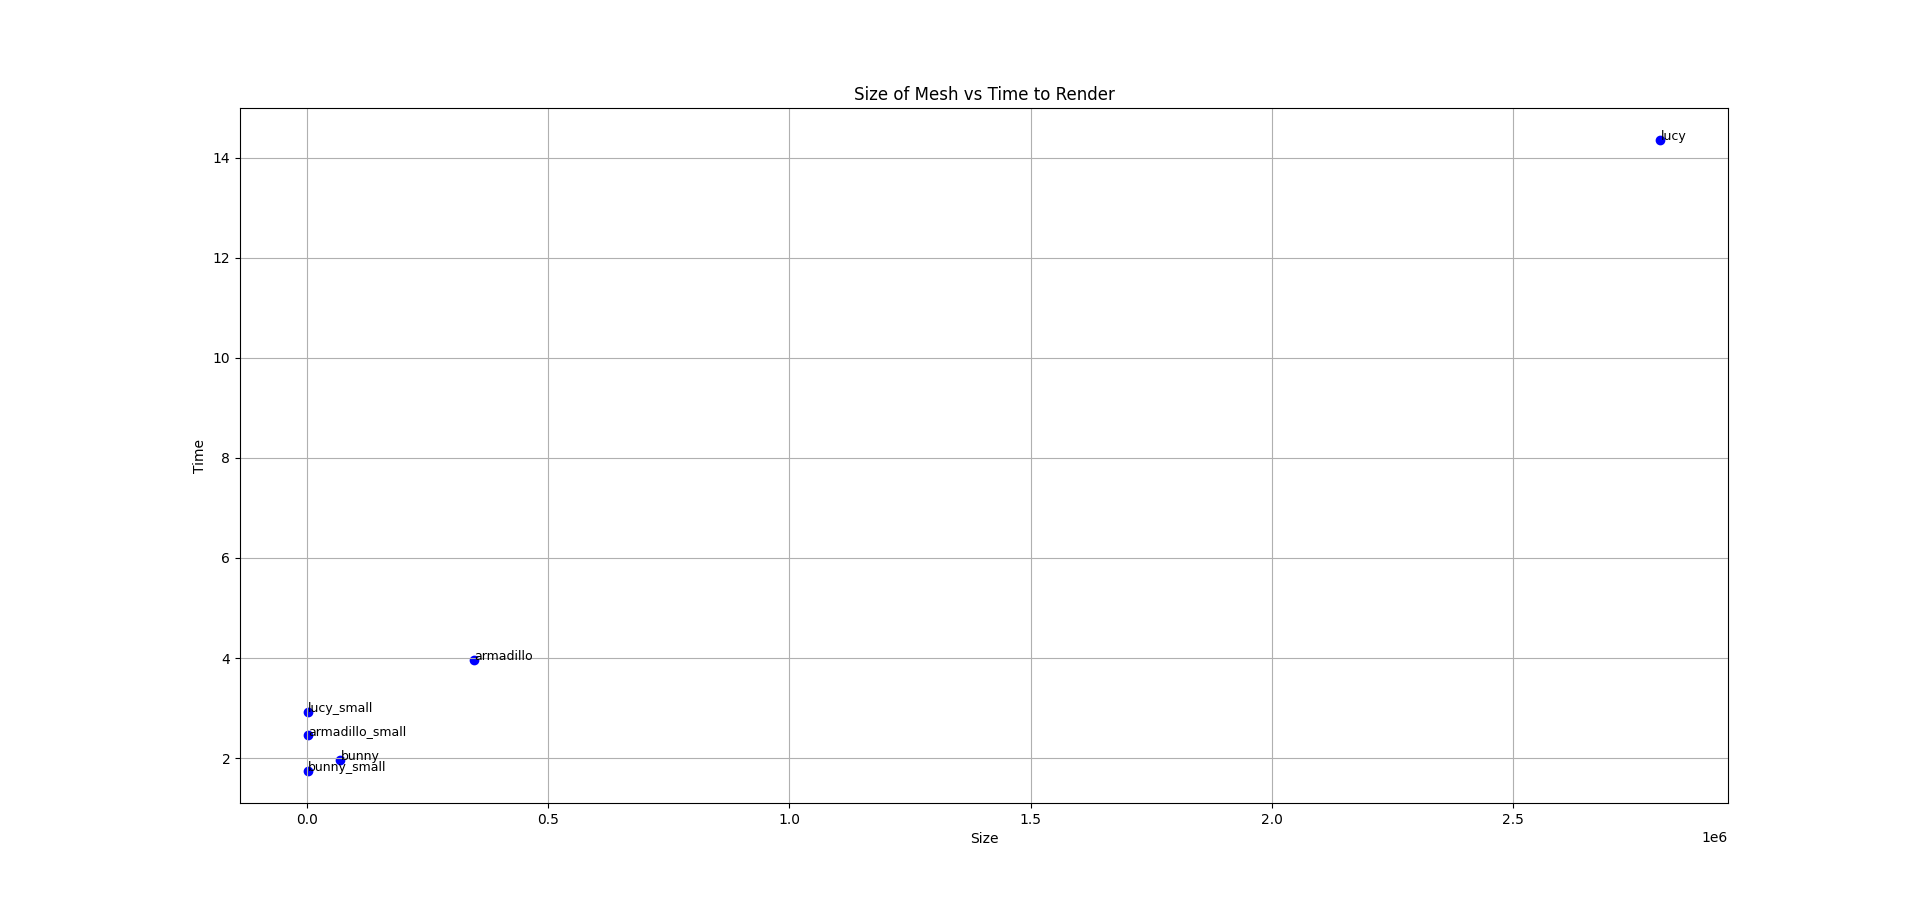
\includegraphics[width=\linewidth]{Figure_1.png}
\end{figure}


As expected, we can observe a sub-linear relationship between the number of triangles and the render time.


\end{document}
